
%---------------------------------------------------------------
\chapter{The P4 Language}
%---------------------------------------------------------------

\begin{chapterabstract}
	\dots in which we delve into the syntax and semantics of \acrshort{p4},
	explain its use cases, and discuss the differences to conventional programming
	languages.
\end{chapterabstract}

One of the original motivations behind \acrshort{p4} was the need for
restriction. While other \acrlong{dsl}s, such as Click\todo{citation}, existed
at the time, their embeddings within general-purpose programming languages made
it difficult to analyze data dependencies crucial for scheduling parallel
execution. The expressiveness of a language complicates its efficient
compilation. In the words of Robert Harper,

\begin{displayquote}
	\textit{The expressive power of a programming language arises from its
	strictures and \emph{not} from its affordances.}

	-- Robert Harper, \citedate*{pfpl1oplss2019} \cite{pfpl1oplss2019}
\end{displayquote}

Rather than embedding \acrshort{p4} in an existing language, these
considerations motivated a clean-slate design. However, to understand why is
packet processing any different from tasks suited to general-purpose programming
languages, we need to familiarise ourselves with the switching architecture.

%----------------------------%
\section{What's in a switch}
%----------------------------%

In the following text, we choose to use \emph{switch} to mean a general packet
forwarding device. Examples of switches are

A network switch
\todo[inline]{need a readable description of this \& network routing, also
citations in the text below}

Traditionally, these devices were examples of fixed-function hardware. Various
networking protocols were implemented directly in circuitry, which made them
efficient, but inflexible. It is impossible to reconfigure a fixed-function
\acrshort{asic} to process a protocol it was not explicitly designed for in
advance. If a new, backward-incompatible version of a given protocol emerges, or
if a hardware error is found in the chip, the network administrators need to
perform a costly hardware replacement in order to support, respectively
circumvent it. Moreover, fixed-function hardware design is a lengthy and
resource-intensive process. It may take several years before an updated
fixed-function chip hits the market.

The innovation of recent years is the introduction of \emph{programmable}
network processors, which can change the set of supported protocols on the fly.
These are similar to \acrshort{fpga}s in their reconfigurability, but
specialised to packet switching and routing, which makes them more efficient. A
programmable network switch has typically no prior knowledge of networking
protocols but contains efficient circuitry for parsing and pattern-matching in
order to support arbitrary\footnote{To some degree of complexity supported by
the circuit.} protocols uploaded to the chip as microcode. While programmable
networking hardware does incur a penalty for reconfigurability, when it comes to
efficiency, it sits between fixed-function devices and completely general-purpose
solutions.

Other implementations of packet switching are also common. The already mentioned
\acrlong{fpga}s can be programmed to simulate programmable or fixed-function
networking hardware, and thus allow an even higher degree of flexibility.
Naturally, \acrshort{fpga}s are less efficient than the circuits they simulate.
Finally, there are software switches, programs for widespread processor
architectures and operating systems, such as x86 and Linux. A software switch
represents the peak of flexibility, programmability, and requires no special
hardware other than what is already commonly present in conventional computers.
Purely software-based solutions cannot compete in energy efficiency with any of
the other approaches, but are often useful for testing and in small-scale
networks.

\begin{figure}[t]
	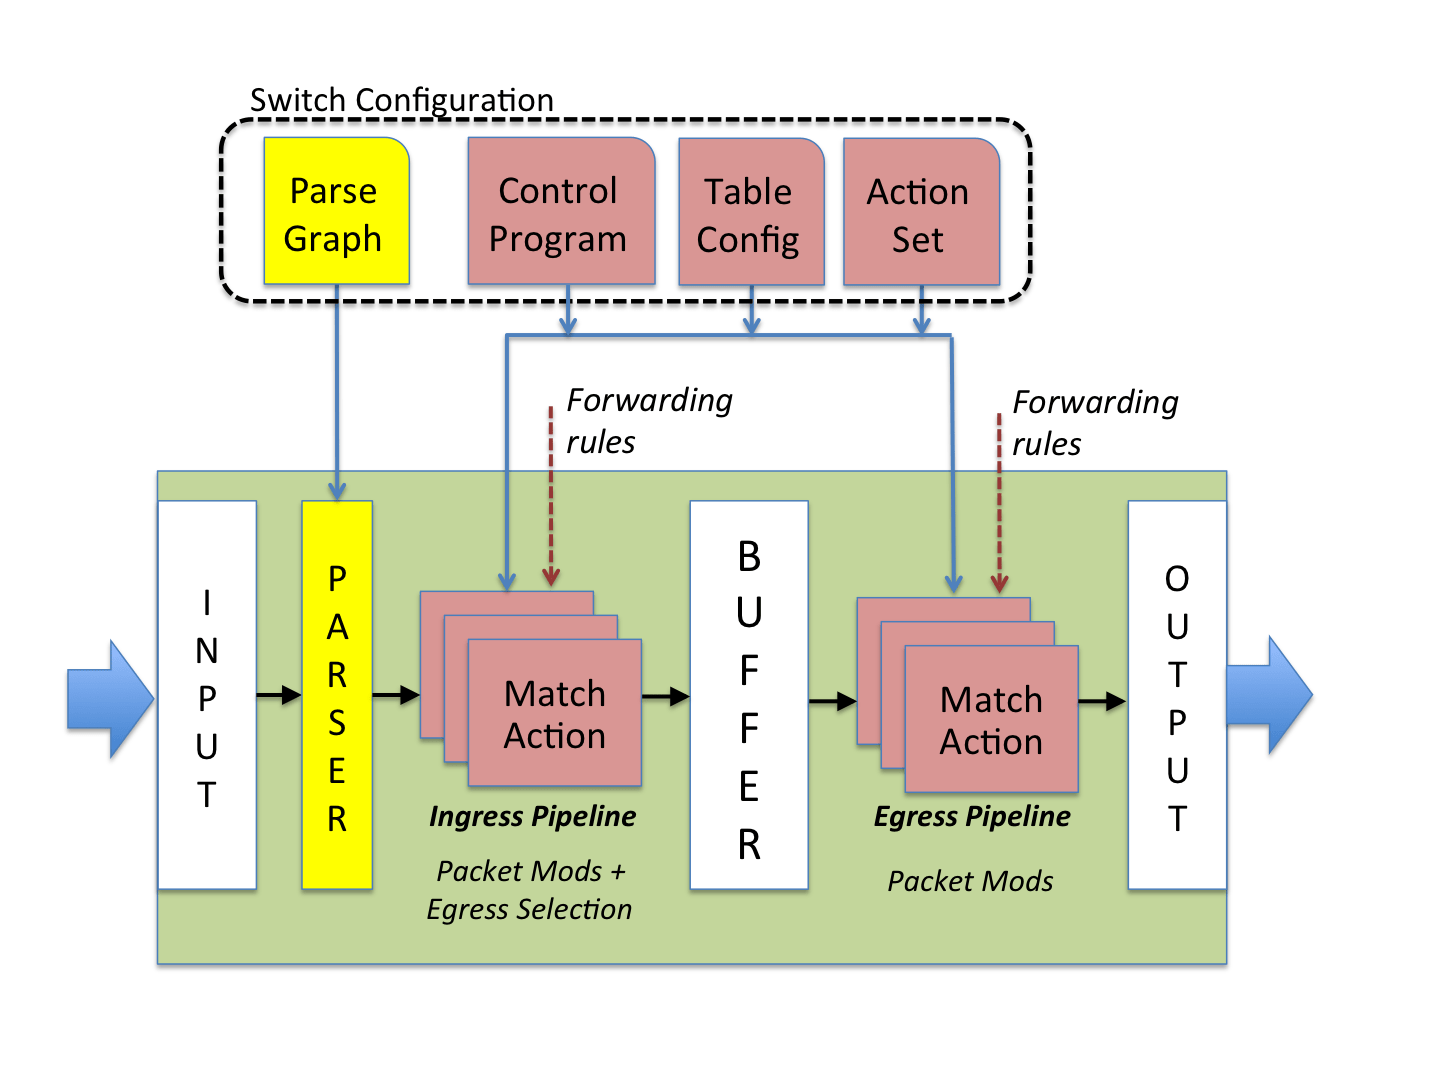
\includegraphics[
		trim={2.0cm 4.3cm 4.0cm 3.3cm}, % left bottom right top (insane, I know)
		width=1.00\textwidth
	]{resources/abstract-forwarding-model.png}
	\caption{The original \acrshort{p4}\textsubscript{14} abstract forwarding
	model, taken from \cite{p4original}.}
	\label{fig:abstract-forwarding-model}
\end{figure}

To support network configurations regardless of their physical implementation,
the original \acrshort{p4} paper defines the target-independent \emph{abstract
forwarding model}, outlined in Figure~\ref{fig:abstract-forwarding-model}. This
model assumes an end-to-end pipeline split into \emph{ingress} and \emph{egress}
parts. An arriving packet is first parsed to recognize the headers present
therein. These headers then travel through the pipeline's \emph{match-action
units}. A match-action unit performs limited pattern-matching and rewriting on
the parsed packet header. This part of the pipeline is partially configured at
runtime by the control plane. Forwarding rules defined in software are uploaded
to the network device.

\todo[inline]{all this needs a much better explanation! it's crucial for
understanding the P4 way of doing things.}

The model assumes that the payload is handled separately by the device and is
not available for pattern-matching.

\todo[inline]{finish the model description, mention deparsers, explain metadata}

A lifetime may end early if the packet is dropped during processing. Dropping is
indicated by mutating metadata.

%--------------------------%
\section{The \pfs language}
%--------------------------%

\begin{figure}[t]
	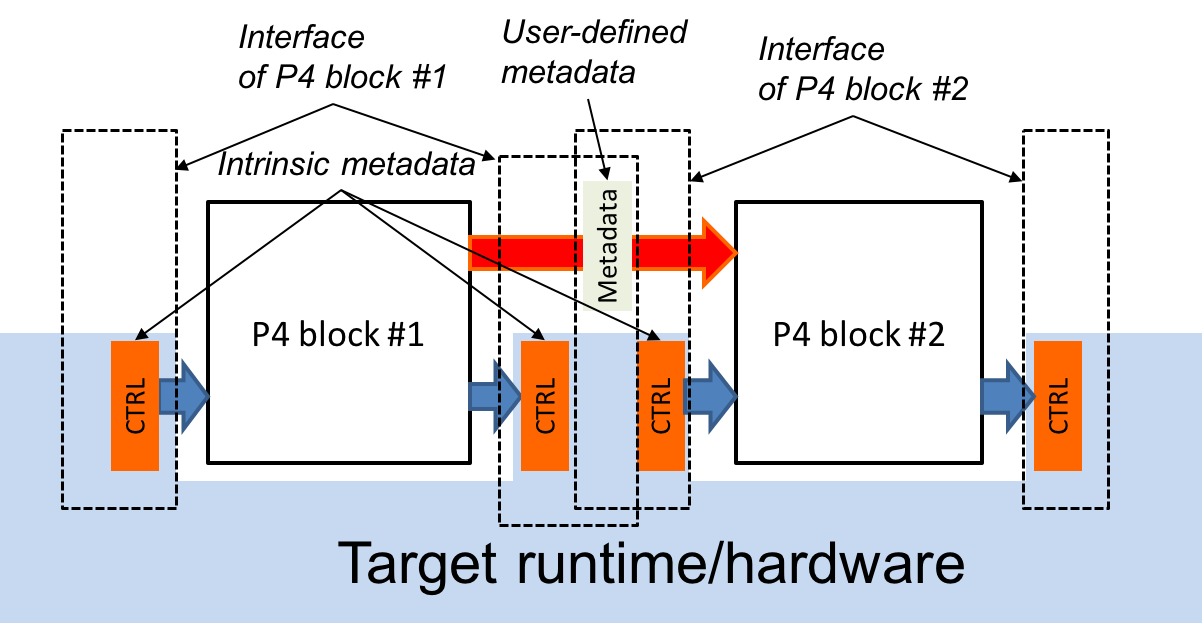
\includegraphics[width=1.00\textwidth]{resources/p4_16-architecture-model.png}

	\caption{\pfs program interfaces for an abstract architecture with two
	programmable blocks, taken from \cite{p416:v123:spec}.}
	\label{fig:arch-model}
\end{figure}

\acrshort{p4} is not a programming language for von Neumann architectures. The
abstract model assumes the target machine to be some sort of network processor
with programmable blocks embedded in a static pipeline.
Figure~\ref{fig:arch-model} illustrates such a machine and highlights the
interfaces of the \acrshort{p4} program.

A \acrshort{p4} program specifies a mapping of vectors of bits -- a bit\-vector
endomorphism. Every \acrshort{p4} program terminates; the language has no
looping constructs and no recursion, a compiler can thus determine the precise
maximum runtime of a program statically.

\todo[inline]{in discussing the subpar nature of the spec, include examples of
	mistakes.
	\href{https://p4.org/p4-spec/docs/P4-16-v-1.2.3.html\#sec-minsizeinbits}
	{compile-time size determination} mentions ``\emph{Each of these method
	calls evaluate to compile-time known values that return the minimum size in
	bits required to store the expression,}'' clearly forgetting to take the
	\texttt{maxSize*} functions into account}

\subsection{Syntax}

\todo[inline]{
	describe headers and their relation to structs, explain annotations
}

% relevant p4 spec sections

% 6.1.   Syntax and semantics
% 6.1.1. Grammar
% 6.1.2. Semantics and the P4 abstract machines
% 6.2.   Preprocessing
% 6.2.1. P4 core library
% 6.3.   Lexical constructs
% 6.3.1. Identifiers
% 6.3.2. Comments
% 6.3.3. Literal constants
% 6.4.   Naming conventions
% 6.5.   P4 programs
% 6.5.1. Scopes
% 6.5.2. Stateful elements
% 6.6.   L-values
% 6.7.   Calling convention: call by copy in/copy out
% 6.7.1. Justification
% 6.7.2. Optional parameters
% 6.8.   Name resolution
% 6.9.   Visibility

\pfs syntax is reminiscent of imperative programming languages in the C family.
It uses prefix notation for typed bindings, braces for lexical scoping blocks,
and semicolons to separate statements. However, instead of general-purpose
procedures, the top level constructs for executable code are mainly controls,
parsers, and actions. These will be explained in detail in this section.

\subsubsection*{\texttt{extern} objects and functions}

Before diving into the bulk of the syntactical forms that dominate user-written
\acrshort{p4} code, we need to introduce the general concept of
\texttt{extern}s. These special objects and functions were already present in
\acrshort{p4}\textsubscript{14} version 1.1. \pfs fully embraced these
constructs, which helped to both simplify and generalize the language.

\texttt{extern} objects and functions describe interfaces to facilities provided
by the architecture, as well as certain built-in language
constructs\todo{reference the parser declaration grammar section}. For example,
the \texttt{extern} object in Listing~\ref{lst:p4-extern-cksum} allows
\acrshort{p4} code to utilize a fixed-function checksum unit provided by the
target. The object specifies no implementation for the listed constructors and
methods.

To invoke a method of the checksum unit, the user needs first to
\emph{instantiate} the \texttt{extern} object. This syntactic form is shared
among all types with constructors: \texttt{control} blocks, \texttt{parser}s,
and \texttt{package}s\todo{describe those somewhere}. The effect of an
instantiation is to allocate the corresponding object, binding it to the
specified name.

The compiler is in charge of mapping instances of \texttt{extern}s to the target
architecture. If it does not find a mapping, either because the target does not
support the \texttt{extern} or does not have the resources to fit all its
instances, the compilation fails with an error.

\begin{lstlisting}[
	caption={~An \texttt{extern} object specifying the interface to the target's checksum unit.},
	label=lst:p4-extern-cksum,
	captionpos=t,
	tabsize=4,
	float,
	abovecaptionskip=-\medskipamount,
	belowcaptionskip=\medskipamount,
	language=p4
]
extern Checksum16 {
	Checksum16();              // constructor
	void clear();              // prepare unit for computation
	void update<T>(in T data); // add data to checksum
	void remove<T>(in T data); // remove data from existing checksum
	bit<16> get(); // get the checksum for the data added since last clear
}
\end{lstlisting}

\subsubsection*{Functions and parametrized code}

Functions in \acrshort{p4} come in several flavours. The first kind is known as
\emph{function declarations} and is perhaps the closest relative of procedures
in conventional imperative programming languages. The major difference is that
all parameters to a \acrshort{p4} function need to include a \emph{direction}.

\begin{description}
	\item[parameter direction] is either \texttt{in}, \texttt{out}, or
	\texttt{inout}. \texttt{in} indicates a read-only parameter with a defined
	value, \texttt{out} indicates a read-write parameter whose value is
	initially undefined upon entering the function body, and \texttt{inout}
	indicates a read-write parameter with a defined value.
\end{description}

Only l-values\todo{what are those?} can be passed as \texttt{out} and
\texttt{inout} parameters. The execution of the function call can change the
value of an \texttt{out} or \texttt{inout} parameter's corresponding l-value.
Note that \acrshort{p4} functions can combine \texttt{out} parameters and return
values.

Parameter directions are \acrshort{p4}'s way of introducing a limited form of
references, themselves a principled approach to pointers. Parametrized
\acrshort{p4} code follows a copy in / copy out calling convention, which makes
functions easy to reason about and limits side effecting behaviour of
\texttt{extern} methods. We will discuss this later in ?\todo{reference here}

.
\todo[inline]{subsubsubsection?}

Another construct for parametrized code are \emph{parser declarations}. A
\acrshort{p4} parser describes a \acrlong{fsm} whose job is to recognize valid
packets and load their headers into the storage facilities of the target. Parser
declarations define all the states of the \acrshort{fsm}, except the implicit
built-in \texttt{accept} and \texttt{reject} states further described in the
semantics section\todo{reference here}. Each parser has to contain at least the
initial \texttt{start} state. During parsing, the parser can manipulate local
state\todo{context?} in the form of variables and \texttt{extern}
instantiations. These are defined directly in the parser declaration block,
before listing any states, meaning that the type of this local context is
statically known and independent of the state the parser may appear in at
runtime. In other words, parser declarations follow lexical scoping.

States can introduce lexically-scoped local variables, but not additional
\texttt{extern}s. Other statements like conditionals, assignments, or method
calls are also allowed. The specification explicitly points out that specific
target architectures can place restrictions on the set of constructs and
operations a programmer can use within a parser.

\pfs parser declarations unrestricted by the target architecture may appear very
similar to regular imperative code. However, the important distinction between a
parser and other function-like constructs in the \pfs language are data
extraction, pattern-matching, error handling, and state transitions.

Data extraction moves information from the input packet into memory available
for pattern-matching further down the pipeline, typically registers or similar
containers. To facilitate this operation, the \acrshort{p4} core library
contains an intrinsic\todo{established term?} \texttt{extern}\todo{we should
definitely change this and the plural into a command} definition called
\texttt{packet\_in} which represents incoming packets. This special
\texttt{extern} cannot be manually instantiated\todo{make sure we explain
instantiation prior to this. Maybe externs should be described first in the
syntax section?}, but it is instantiated implicitly for every parser
parameter\todo{arg vs param} of type \texttt{packet\_in}. This allows parser
states to invoke the methods of this \texttt{extern}, shown in
Listing~\ref{lst:p4-prsr-packet-in}.

\begin{lstlisting}[
	caption={~The intrinsic \texttt{extern} that facilitates data extraction.},
	label=lst:p4-prsr-packet-in,
	captionpos=t,
	tabsize=4,
	float,
	abovecaptionskip=-\medskipamount,
	belowcaptionskip=\medskipamount,
	language=c
]
extern packet_in {
	void extract<T>(out T headerLvalue);
	void extract<T>(out T variableSizeHeader, in bit<32> varFieldSizeBits);
	T lookahead<T>();
	bit<32> length();  // This method may be unavailable in some architectures
	void advance(bit<32> bits);
}
\end{lstlisting}

\begin{lstlisting}[
	caption={~An example of data extraction in a \pfs parser.},
	label=lst:p4-prsr-extract,
	captionpos=t,
	tabsize=4,
	float,
	abovecaptionskip=-\medskipamount,
	belowcaptionskip=\medskipamount,
	language=c
]
struct Result { Ethernet_h ethernet;  /* more fields omitted */ }
parser P(packet_in b, out Result r) {
	state start {
		b.extract(r.ethernet);
	}
}
\end{lstlisting}

An example of extraction of fixed-width data can be seen in
Listing~\ref{lst:p4-prsr-extract}.

Data extraction and computation within parser states subsumes the stateful part
of a \acrlong{fsm}. Because isolated states would not be very useful on their
own, \acrshort{p4} parsers can specify state transitions using the
\texttt{transition} statement. The target of the transition can be either given
statically or computed. A missing \texttt{transition} statement at the end of a
state block implies a transition into the \texttt{reject} state.

Another parser-specific construct facilitates the computation of transition
targets by pattern-matching on extracted data. The \texttt{select} expression
tries to match a value against a number of patterns and evaluates to a state, if
successful. Otherwise, it triggers a runtime error with code
\texttt{error.NoMatch}. The patterns of a \texttt{select} expression can contain
integer literals, bit masks, ranges, don't-care values, tuples (when matching on
multiple values simultaneously), or, on some architectures, \textit{parser value
sets} specified at runtime by the control plane.\todo{one snippet to rule them
all, one snippet to find them, one snippet to bring them all and in the \LaTeX{}
bind them.}

While error-handling already happens implicitly in \texttt{select} expressions,
the \texttt{verify} statement, defined in Listing~\ref{lst:p4-prsr-verify},
allows the programmer to ergonomically check arbitrary assertions about the
parsed data. Passing \texttt{false} as the first argument to \texttt{verify}
immediately transitions to the \texttt{reject} state, setting the parser error
to the code given as the second argument. Otherwise, execution proceeds with the
next statement.

\begin{lstlisting}[
	caption={~The interface of the \texttt{verify} built-in.},
	label=lst:p4-prsr-verify,
	captionpos=t,
	tabsize=4,
	float,
	abovecaptionskip=-\medskipamount,
	belowcaptionskip=\medskipamount,
	language=c
]
extern void verify(in bool condition, in error err);
\end{lstlisting}

\begin{figure}\centering
	\begin{tikzpicture}[
		->,
		>=stealth,
		shorten >=1pt,
		auto,
		node distance=1cm,
		semithick
	]
		\tikzstyle{every state}=[fill=white,draw=black,text=black,minimum size=2em]
		\tikzstyle{cloud}=[draw=gray!20,circle,fill=gray!10,minimum height=2em]
		\tikzstyle{rejecting}=[state,double,minimum size=2em]

		\node[state] (start) {$\text{start}$};
		\node[state, below=of start] (q2) {};
		\node[state, left=of q2] (q1) {};
		\node[state, below=of q1] (q3) {};
		\node[state, below=of q2] (q4) {};
		\node[state, right=of q4] (q5) {};
		\node[state, accepting, below=1.5cm of q4] (accept) {$\text{accept}$};
		\node[rejecting, below=1.5cm of q3] (reject) {$\text{reject}$};

		\begin{pgfonlayer}{background}
			\node[cloud,fit=(q1)(q2)(q3)(q4)(q5)(start),inner sep=2pt] (cloud) {};
		\end{pgfonlayer}

		\path
			(start) edge          (q2)
			(q1)edge              (q2)
				edge              (q3)
			(q2)edge              (q4)
			(q3)edge              (q4)
				edge              (reject)
			(q4)edge              (q5)
				edge              (accept)
			(q5)edge              (accept)
			(q5)edge [bend right] (q3);
	\end{tikzpicture}
	\caption{An abstract overview of a \acrshort{p4} parser. The states inside
	the grey circle are accessible to user code.}
	\todo[inline]{add a loop}
	\label{fig:parser-overview}
\end{figure}


\begin{lstlisting}[
	caption={~A function declaration in \pfs.},
	label=lst:p4-fun,
	captionpos=t,
	tabsize=4,
	float,
	abovecaptionskip=-\medskipamount,
	belowcaptionskip=\medskipamount,
	language=c
]
bit<32> max(in bit<32> left, in bit<32> right) {
	return (left > right) ? left : right;
}
\end{lstlisting}

\todo[inline]{subparsers, header stacks}

\todo[inline]{we should really reorganise this to use bigger headings, this way
the individual constructs are lost in the text!}

While parsers execute at the very frontier of the pipeline, the bulk of packet
processing happens in match-action units\todo{previously mentioned?}.
\acrshort{p4} has another parametrized construct for expressing entire sequences
of pattern-matching and rewriting steps: \texttt{control} blocks\todo{Add an
example control block listing}.

A control block has a name and can take type and value parameters. The body of a
control block begins with declarations of constants, variables, and
instantiations. It follows with definitions of \emph{\texttt{action}s}.

A \acrshort{p4} action\todo{example listing} is a piece of code that directly
manipulates packet headers. At a first glance, actions should be immediately
familiar to imperative programmers, since they resemble functions with no return
value. Their bodies are each comprised of a series of statements. These are
executed sequentially\footnote{At least from the perspective of the
programmer.}. There are two important restrictions on action parameter lists.

\begin{enumerate}
	\item Parameters with no direction must all come at the end of the parameter
	list. These directionless parameters indicate \emph{action
	data}\todo{explain what that is}.
	\item Action parameters cannot have \texttt{extern} types.
\end{enumerate}

The second major \acrshort{p4} construct that appears exclusively\todo{right?}
within control blocks are \emph{tables}. Whereas an action specifies the
operations performed on packet headers when pattern-matching succeeds, a table
informs a match-action unit of the target how to perform the pattern-matching
and what actions to invoke.

Functional programmers will note that tables and actions together seem like a
low-level decomposition of pattern-matching from Haskell or Scala. This is a
good analogy, except that, whereas pattern-matching constructs in a programming
language are typically fixed at compilation time, \acrshort{p4} tables are
configurable at runtime by the control plane. Furthermore, \acrshort{p4}'s
pattern-matching operates at the bit level and offers certain string-like
facilities.\todo{this whole thing should be like an aside or something}

A \texttt{table} declaration is simultaneously an instantiation in the enclosing
control block. The declaration lists various properties of the table, given as
key-value pairs. It has at least the mandatory \texttt{key} and \texttt{actions}
properties, which specify an expression used for computing the lookup key and
the set of actions the table can invoke, respectively. A table declaration can
optionally also include \texttt{default\_action}, \texttt{entries}, and/or
\texttt{size} properties, which specify the action invoked when no other actions
match\footnote{The \texttt{default\_action} property defaults to the built-in
\texttt{NoAction} when not specified.}, a predefined set of entries for the
table, and the desired size for the table. Compilers can choose to extend this
standard set of properties with additional target-specific key-value pairs.

The programmer can optionally declare table properties as \texttt{const}. This
keyword ensures that the control plane cannot change the property's value at
runtime. Somewhat confusingly, some properties are implicitly \texttt{const},
including the standard properties \texttt{key}, \texttt{actions}, and
\texttt{size}. On these, the \texttt{const} keyword has no effect.

\todo[inline]{some sort of heading for keys here}

\begin{description}

\item[\texttt{key}] The \texttt{key} table property specifies the scrutinee of
pattern-matching. Grammatically, the key is a sequence of rows where each row
contains the expression to match on, the kind of matching to perform, and a list
of optional annotations.

The possible kinds of pattern-matching are \texttt{exact}, \texttt{ternary}, and
\texttt{lpm}, all defined as part of the \texttt{match\_kind} construct in the
core library\todo{do we discuss that prior to this point?}. A
\texttt{match\_kind} behaves like an enumeration, it lists a number of
mutually-exclusive variants. The semantics of the \texttt{match\_kind} variants
is not given, it depends on the compiler and target architecture.

Key elements can be renamed with optional \texttt{@name} annotations to give
them readable names in the control plane \acrshort{api}.

\item[\texttt{actions}] The \texttt{actions} table property lists all the
actions a table can invoke at runtime, separated by semicolons.

The specification mandates that action names of actions in the \texttt{actions}
list have to be distinct. That is, two actions of the same name cannot appear in
the \texttt{actions} list, even if they come from different scopes and could be
disambiguated with fully qualified paths in different contexts.

An overview of the valid and illegal usages of the \texttt{actions} table
property is given in Listing~\ref{lst:p4-table-actions}. The examples highlight
the distinction of action parameters with and without direction. The
directionless parameters, also known as \emph{action data}, are used to
communicate data between the control plane and the data plane at runtime, and
therefore cannot be bound in the \acrshort{p4} program. Haskell enthusiasts may
note that the distinction between compile time and runtime -bound values is
somewhat reminiscent of second-class functions.

\begin{lstlisting}[
	caption={~Use of the \texttt{actions} table property in \pfs.},
	label=lst:p4-table-actions,
	captionpos=t,
	tabsize=4,
	float,
	abovecaptionskip=-\medskipamount,
	belowcaptionskip=\medskipamount,
	language=c
]
action a(in bit<32> x) { /* body omitted */ }
bit<32> z;
action b(inout bit<32> x, bit<8> data) { /* body omitted */ }
table t {
	actions = {
		// a;
		//  - illegal, x parameter must be bound
		a(5);  // binding a's parameter x to 5
		b(z);  // binding b's parameter x to z
		// b(z, 3);
		//      - illegal, cannot bind directionless data parameter
		// b();
		//  -- illegal, x parameter must be bound
		// a(table2.apply().hit ? 5 : 3);
		//   -------------- illegal, cannot apply a table here
	}
}
\end{lstlisting}

\item[\texttt{default\_action}] The \texttt{default\_action} table property
specifies the action invoked when no other actions match. The value of this
property is an expression that invokes the action in question, binding
parameters with directions similarly to an \texttt{actions} list entry. It
introduces an interesting redundancy in the \pfs language, since the programmer
needs to also include the default action in the \texttt{actions} list. Moreover,
the default action and the entry in the list have to be syntactically identical,
except for the directionless parameters. Since there is no action data for the
default action at runtime, the \texttt{default\_action} property has to specify
them all. The directionless parameters are evaluated at compile time.

A table without a \texttt{default\_action} property that does not match a given
packet has no impact on packet processing, it is effectively skipped.

\item[\texttt{entries}] The optional \texttt{entries} property preconfigures a
table's entries. This can serve to either initialize the table or, with the help
of \texttt{const}, turn it into a static construct that cannot be modified on
the control plane side.

\item[\texttt{size}] The optional \texttt{size} property indicates the number of
table entries the table should support at runtime. It is a compile-time known
integer. The interpretation of \texttt{size} depends largely on details of the
target architecture, casting some doubt on why it was included in the core
language. Some targets may require every table to specify a size, others may use
it merely as a hint during dynamic resource allocation, others still may
guarantee that a successfully compiled table can fit at least \texttt{size}
entries. In general, none of these are the case.

\end{description}

Tables can specify additional properties outside of the base set provided by the
\pfs specification\footnote{The specification lists several motivated
examples.}.

\subsection{Semantics}

The semantics of \pfs is defined entirely in terms of abstract machines
executing imperative code. A conforming compiler is free to rewrite the \pfs
program as long as it maintains the observable behaviour of all abstract
machines involved. Unfortunately, the specification gives no formal treatment
of these machines; they are described only in natural language and pseudocode.

\todo[inline]{point out how the language tries to avoid undefined behaviour
and makes arithmetic typing rules saner and safer with no undef. behaviour}


\subsubsection*{Parser abstract machine}

A parser conceptually manipulates a \texttt{ParserModel} data structure.

\begin{lstlisting}[
	caption={~The conceptual model of the state of a \acrshort{p4} parser.},
	label=lst:p4-parser-model,
	captionpos=t,
	tabsize=4,
	float,
	abovecaptionskip=-\medskipamount,
	belowcaptionskip=\medskipamount,
	language=c
]
ParserModel {
    error       parseError;
    onPacketArrival(packet p) {
        ParserModel.parseError = error.NoError;
        goto start;
    }
}
\end{lstlisting}

The meaning of \texttt{accept} and \texttt{reject} states is
architecture-dependent. For example, a rejected packet may be dropped or
passed to the next block of the processing pipeline.

Parser transitions are analogous to \texttt{goto} statements or parameter-less
tail calls.

\subsubsection*{Calling convention}

In order to simplify reasoning about function-like constructs, \pfs follows the
\emph{call by copy in / copy out} calling convention. The specification
describes the exact steps a conforming implementation needs to go follow in
general\footnote{Compiler optimizations could, in specific cases, eliminate some
of these steps, provided prior analysis determines such optimizations correct.}
to evaluate a function call expression.

\begin{displayquote}
	\emph{\begin{enumerate}
		\item Arguments are evaluated from left to right as they appear in the
		function call expression.
		\item If a parameter has a default value and no corresponding argument
		is supplied, the default value is used as an argument.
		\item For each \texttt{out} and \texttt{inout} argument the
		corresponding l-value is saved
		(so it cannot be changed by the evaluation of the following arguments).
		This is important if the argument contains indexing operations into a
		header stack.
		\item The value of each argument is saved into a temporary.
		\item The function is invoked with the temporaries as arguments. We are
		guaranteed that the temporaries that are passed as arguments are never
		aliased to each other, so this ``generated'' function call can be
		implemented using call-by-reference if supported by the architecture.
		\item On function return, the temporaries that correspond to
		\texttt{out} or
		\texttt{inout} arguments are copied in order from left to right into the l-values
		saved in Step 3.
	\end{enumerate}}

	-- \citetitle{p416:v123:spec} \cite{p416:v123:spec}
\end{displayquote}

The calling convention gives function calls\todo{I really need some sort of
universal definition of function-like constructs in p4 that I stick to
throughout the text} a semantics that ensures arguments cannot alias one another
and impure functions cannot hold references to \acrshort{p4} code. This design
is ultimately motivated by the need to control the side effects of
\texttt{extern} functions and methods, which are arbitrarily powerful. The copy
in / copy out calling convention lets compilers reason about programs in the
presence of \texttt{extern}s.

\subsubsection*{Control blocks}

Invoking actions: actions can be invoked either implicitly or explicitly.
Implicit invocations come from tables during match-action processing. Explicit
invocations are calls from \texttt{control} blocks or other \texttt{action}s. In
the explicit invocation case, directionless parameters follow \texttt{in}
parameter semantics.

A table can be invoked explicitly by calling its \texttt{apply} method. This
method is synthetic; it is generated by the compiler. Its return type is a
synthetic \texttt{struct} shared with other actions in a given table. The
compiler generates an \texttt{enum} and a \texttt{struct} for each table, both
of which can be seen in Listing~\ref{lst:p4-table-synthetics}.

\begin{lstlisting}[
	caption={~The synthetic \acrshort{p4} code generated for a table.},
	label=lst:p4-table-synthetics,
	captionpos=t,
	tabsize=4,
	float,
	abovecaptionskip=-\medskipamount,
	belowcaptionskip=\medskipamount,
	language=p4
]
enum action_list(T) {
	// the name of each enum variant is the name of an action
	action_1,
	action_2,
	...
	action_n
}
struct apply_result(T) {
	bool hit;
	bool miss;
	action_list(T) action_run;
}
\end{lstlisting}

Here we see a rationale for the requirement that an action list cannot contain
two actions with the same name. The restriction ensures that the corresponding
enum variants never clash.

The fields in the \texttt{apply\_result(T)} \texttt{struct} indicate whether the
table hit or missed and which action was executed\footnote{\texttt{action\_run}
will be set to the variant corresponding to the table's \texttt{default\_action}
on a table miss.}. The \texttt{hit} and \texttt{miss} fields are
mutually-exclusive, exactly one of them is set when the action returns.

\subsubsection*{The match-action pipeline abstract machine}

The body of a control block is executed serially, as a sequence of imperative
statements.
